% Change numbering of tables and figures
\setcounter{table}{0}
\renewcommand{\thetable}{A\arabic{table}}
\setcounter{figure}{0}
\renewcommand{\thefigure}{A\arabic{figure}}

\section{Figures from Chapter \ref{sec:real-data}}

\begin{figure}[h!]
    \centering
    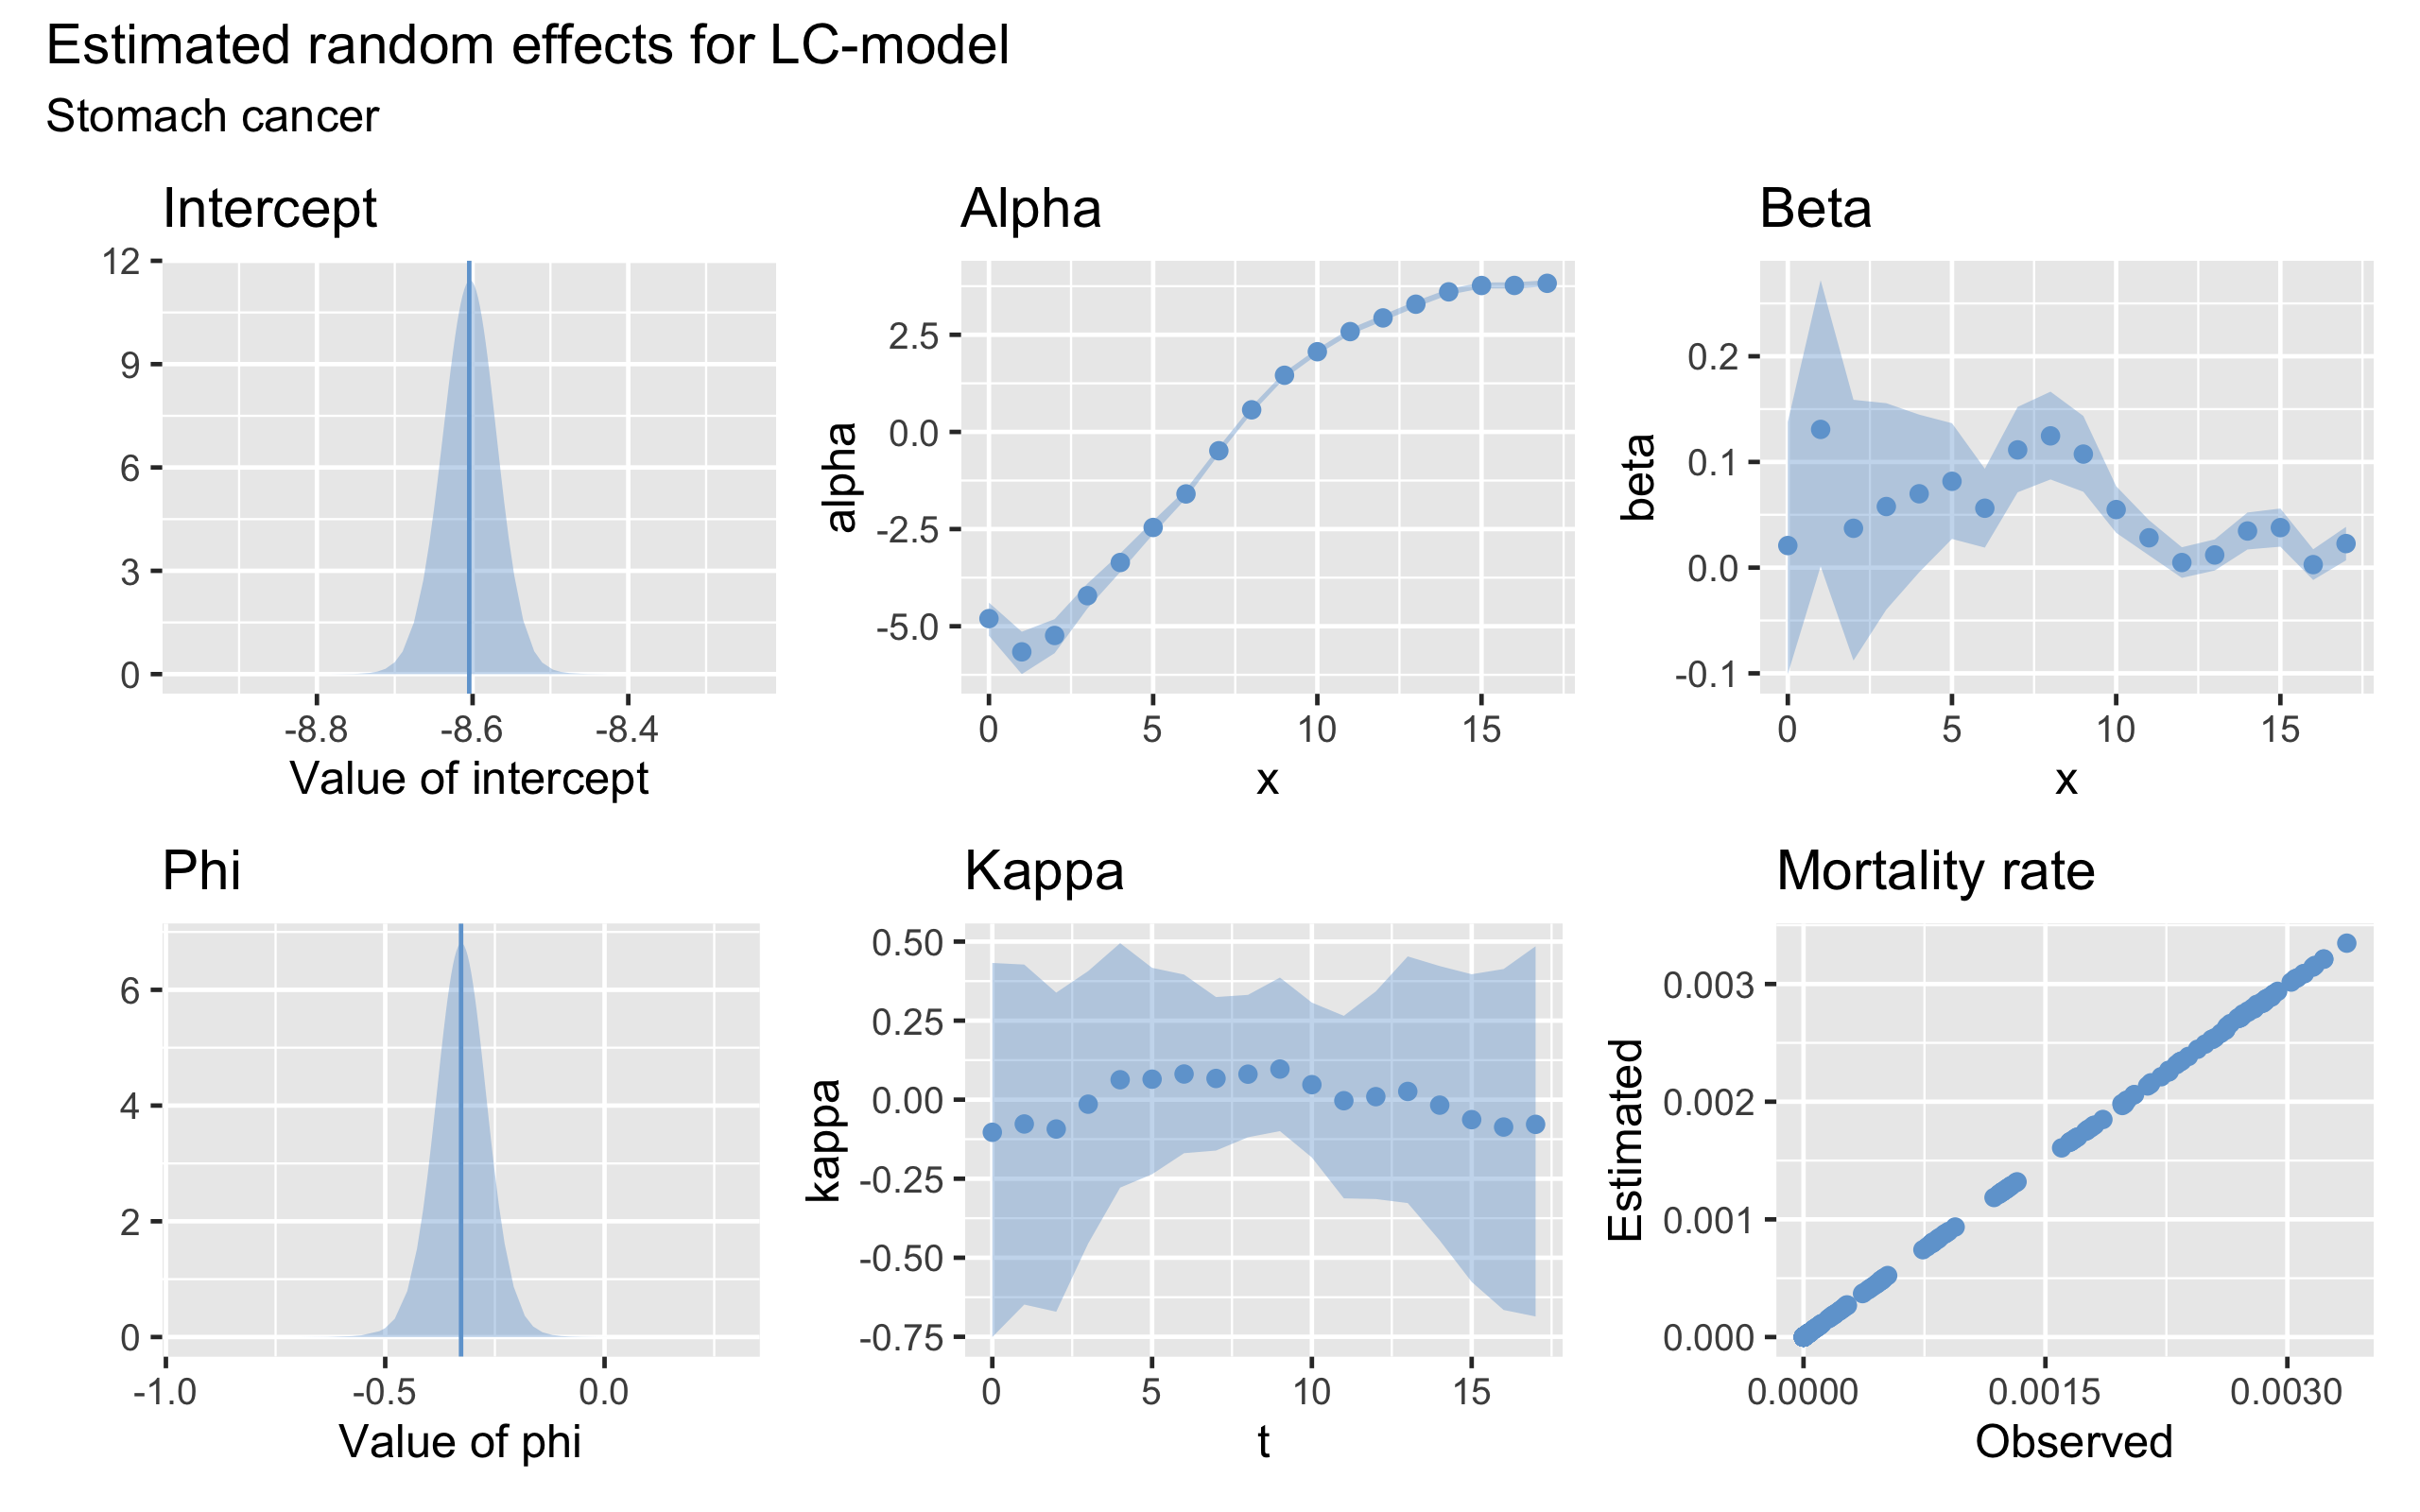
\includegraphics[width=0.85\linewidth]{real-data/real-data-univariate/Figures/uv-full-data-lc-s.png}
    \caption{The estimated effects when fitting the LC-model to stomach cancer data}
    \label{fig:uv-full-data-LC-s}
\end{figure}

\begin{figure}[h!]
    \centering
    \begin{subfigure}[b]{.45\linewidth}
        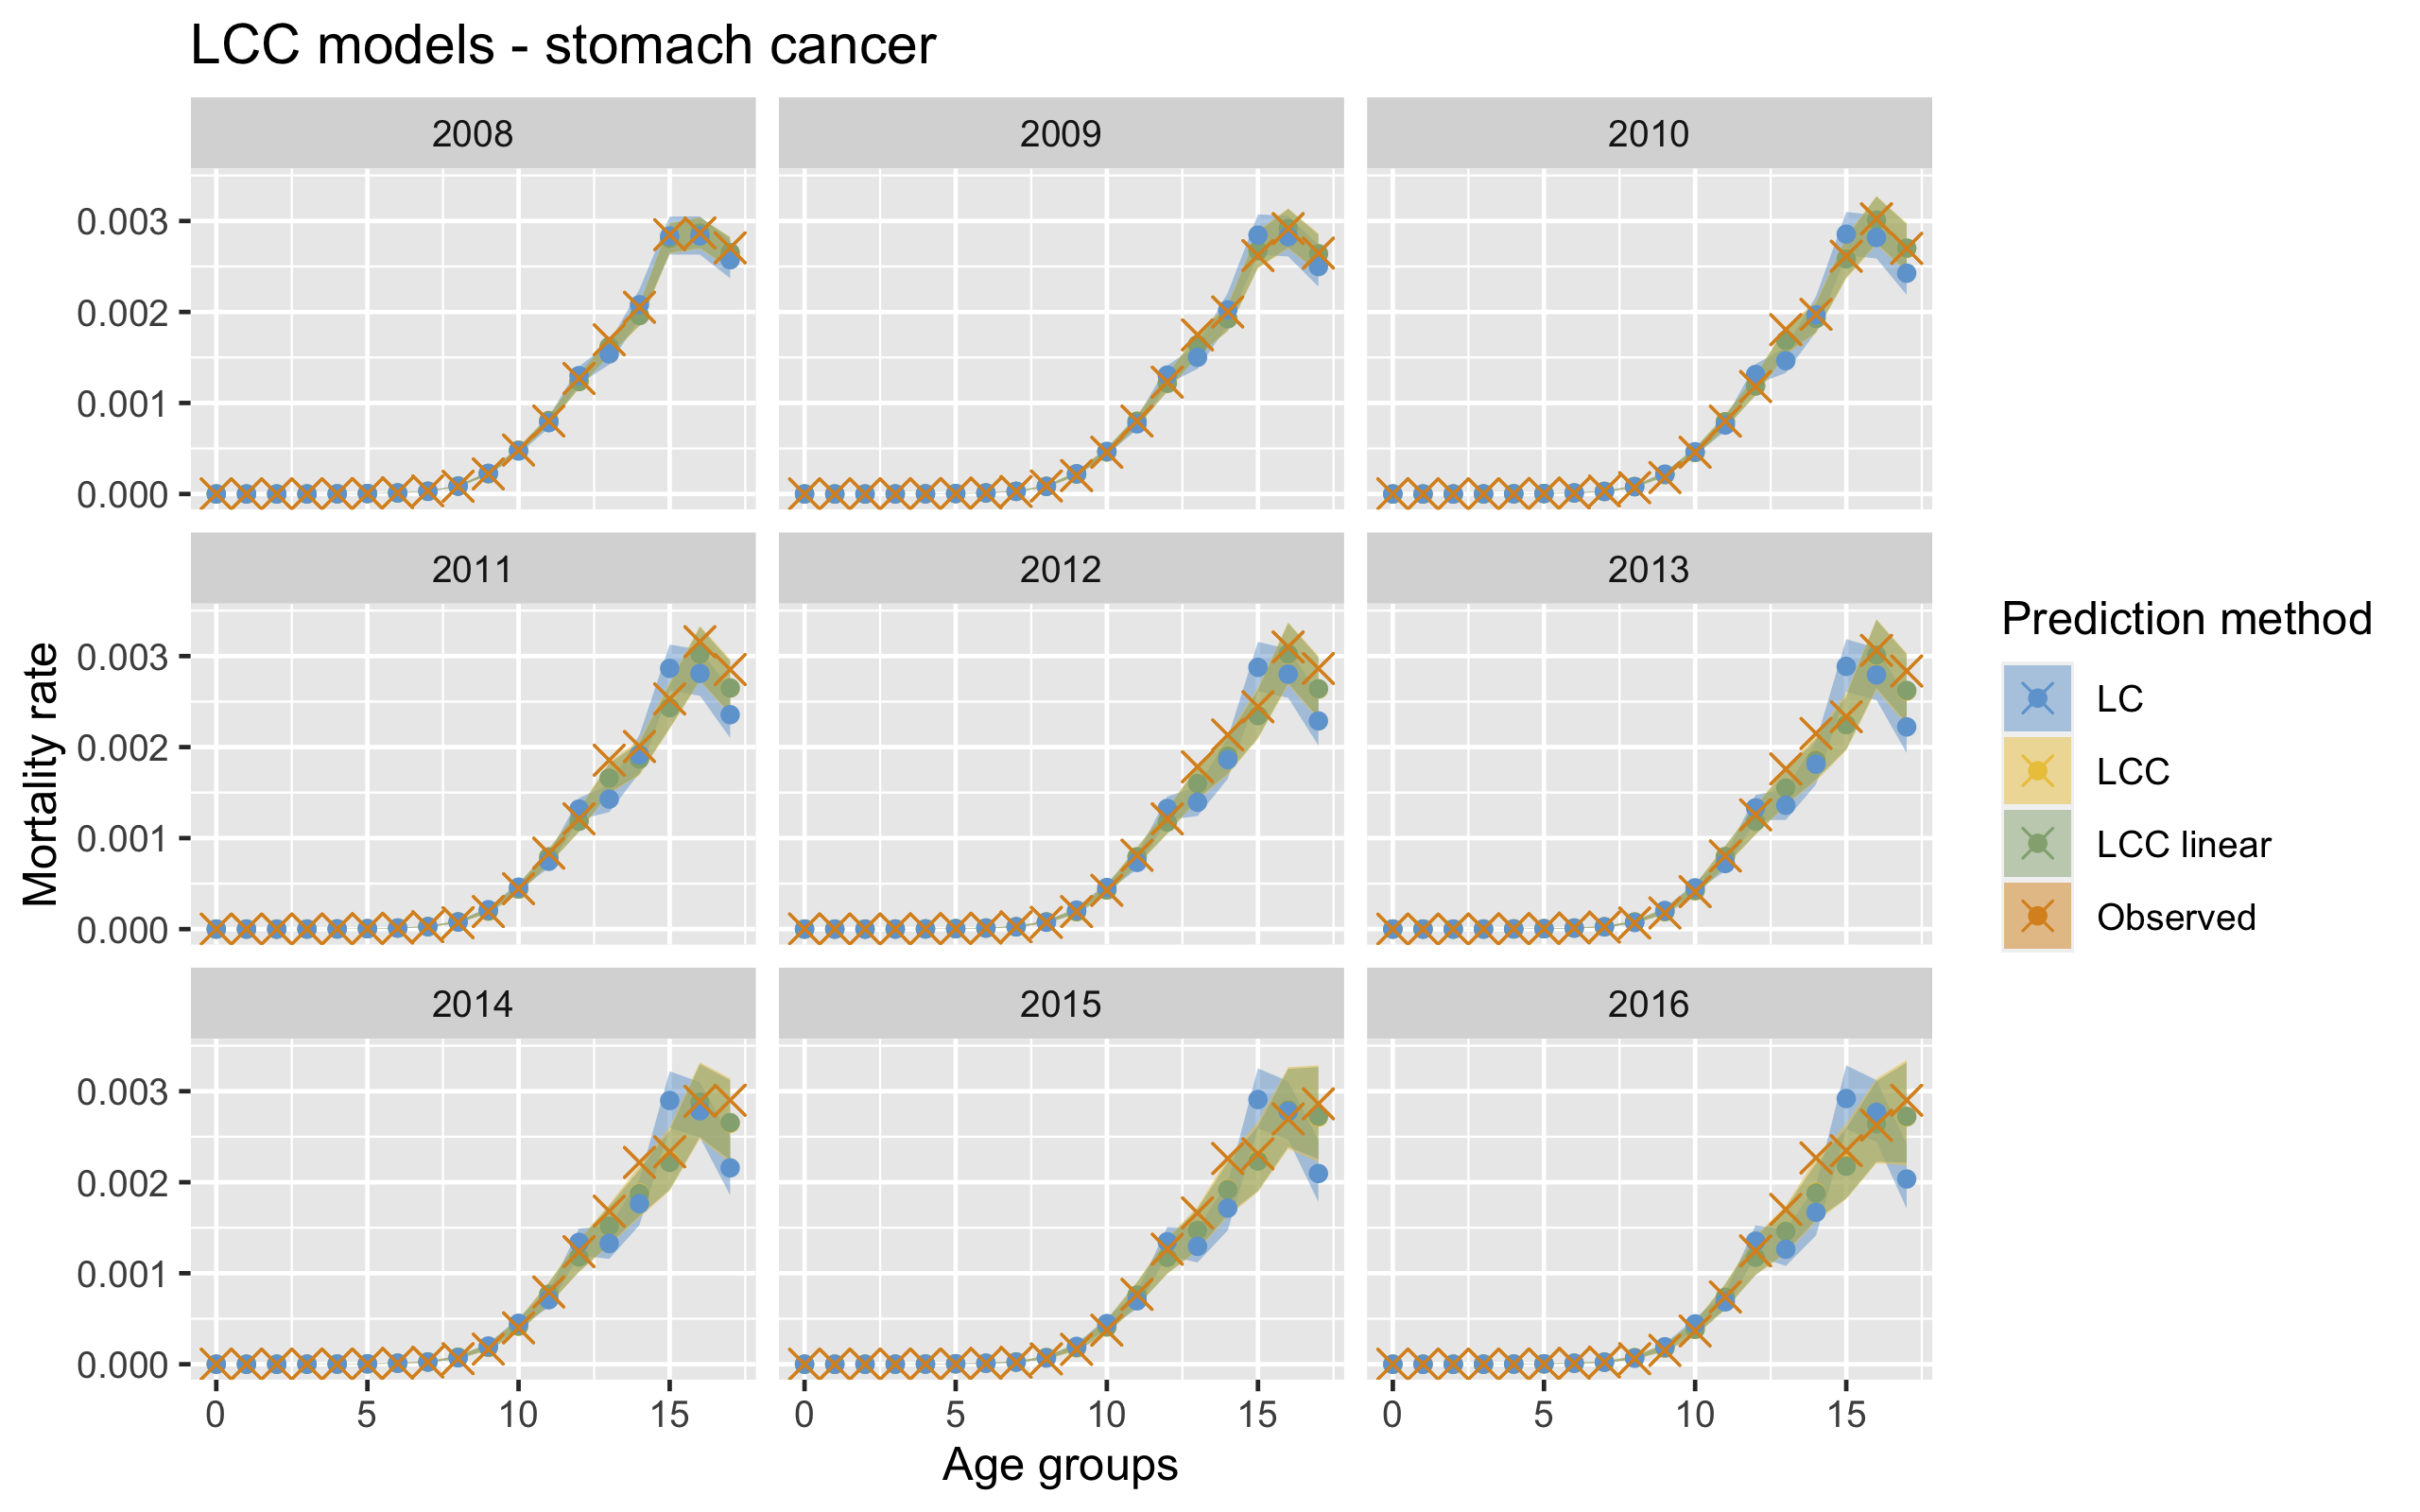
\includegraphics[width=\linewidth]{real-data/real-data-univariate/Figures/univariate-LCC-by-age-stomach.png}
    \end{subfigure}
    \begin{subfigure}[b]{.45\linewidth}
        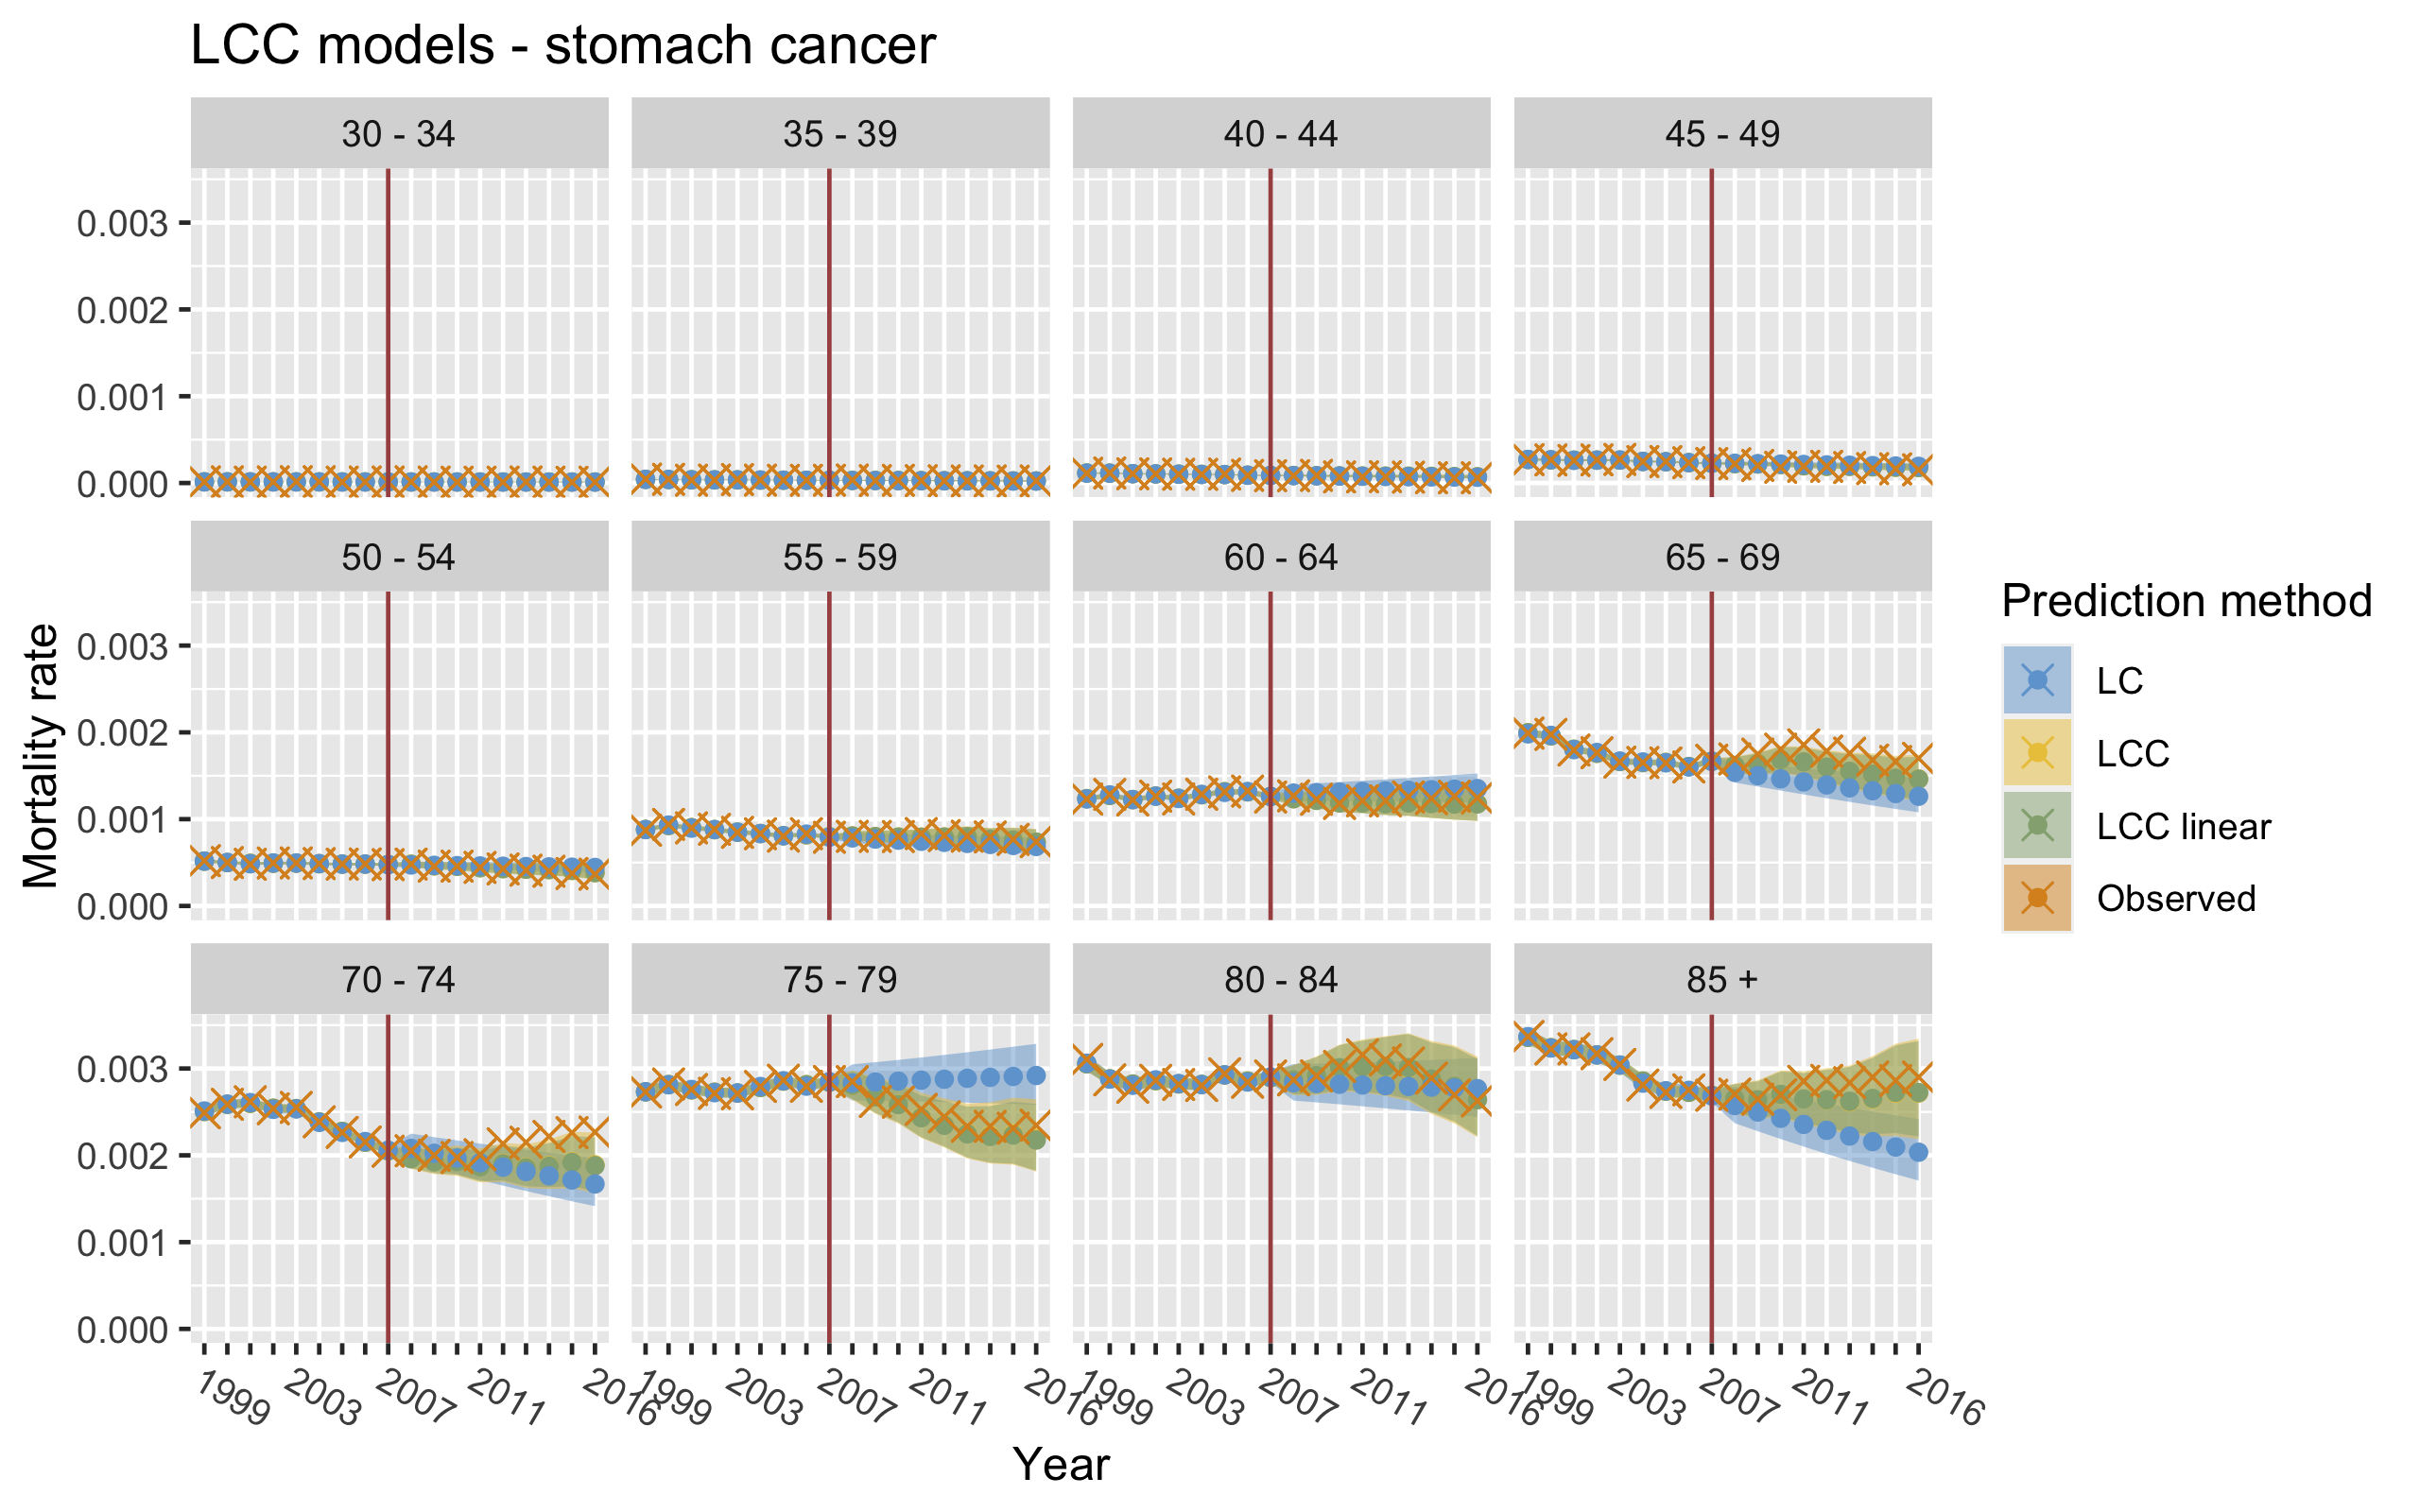
\includegraphics[width=\linewidth]{real-data/real-data-univariate/Figures/univariate-LCC-by-period-stomach.png}
    \end{subfigure}
    \caption{Prediction results from inference with the Lee-Carter types of models on the stomach cancer data set.}
    \label{fig:uv-LCC-stomach}
\end{figure}

\begin{figure}[h!]
    \centering
    \begin{subfigure}[b]{.45\linewidth}
        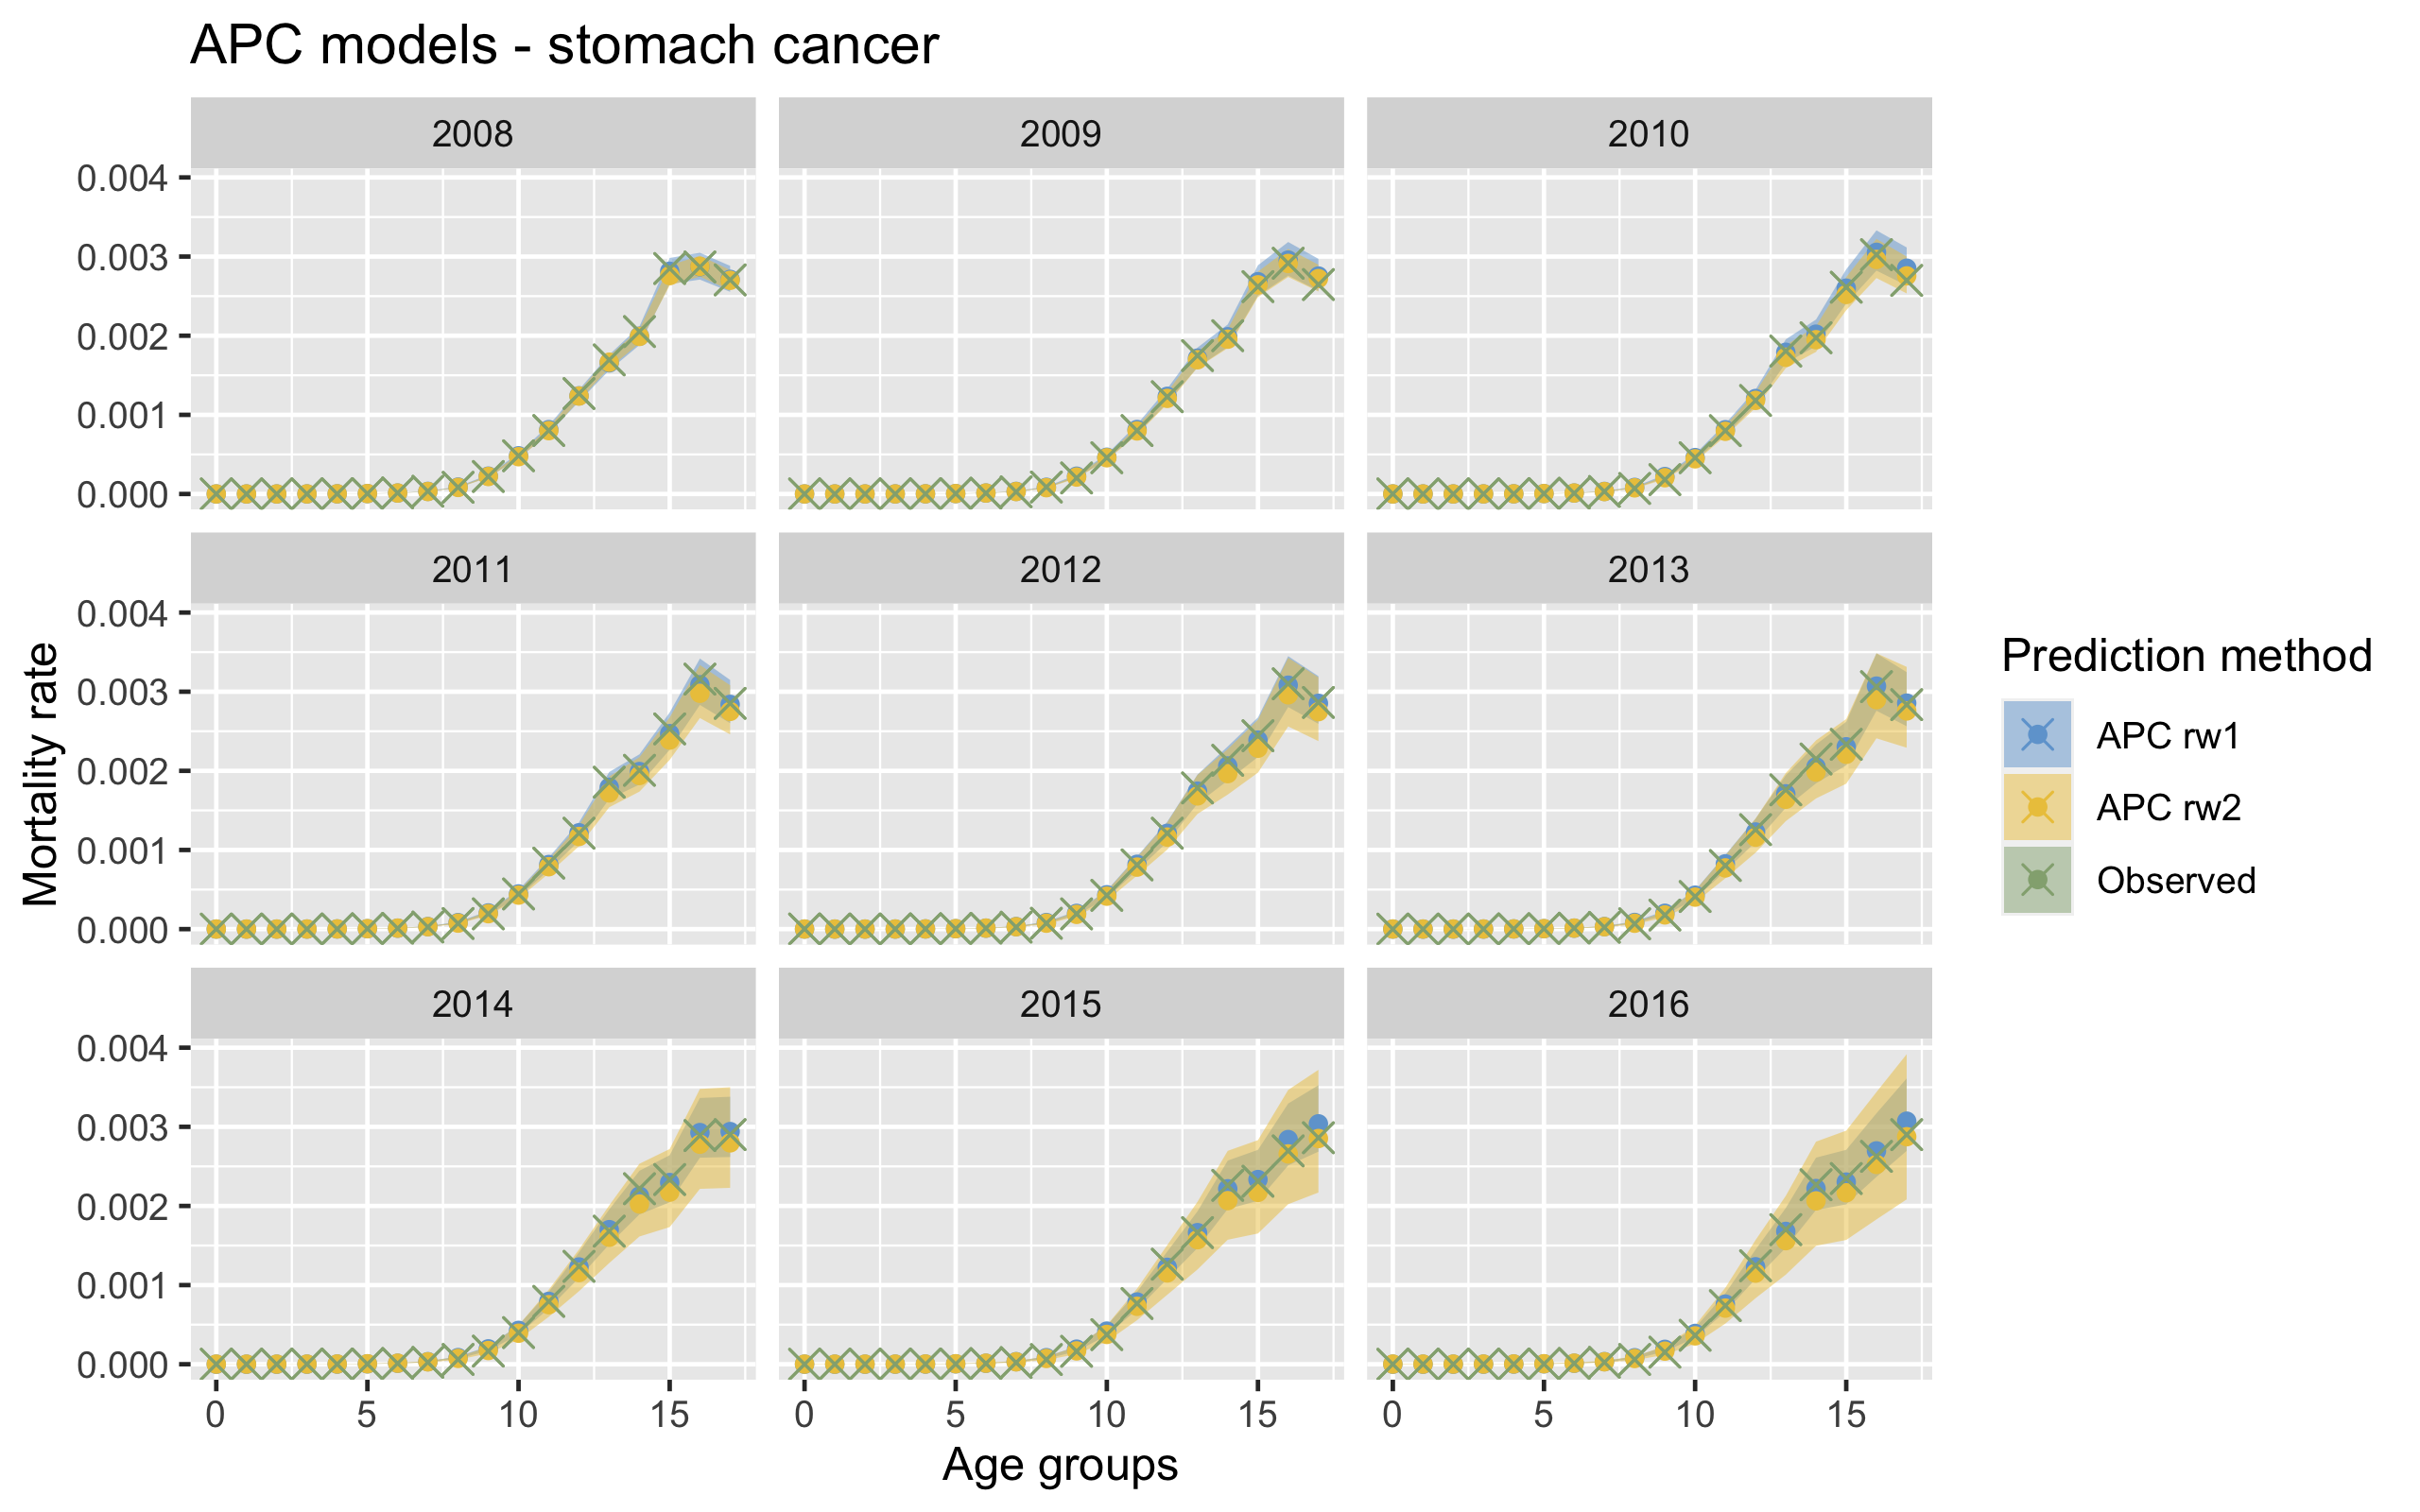
\includegraphics[width=\linewidth]{real-data/real-data-univariate/Figures/univariate-APC-by-age-stomach.png}
    \end{subfigure}
    \begin{subfigure}[b]{.45\linewidth}
        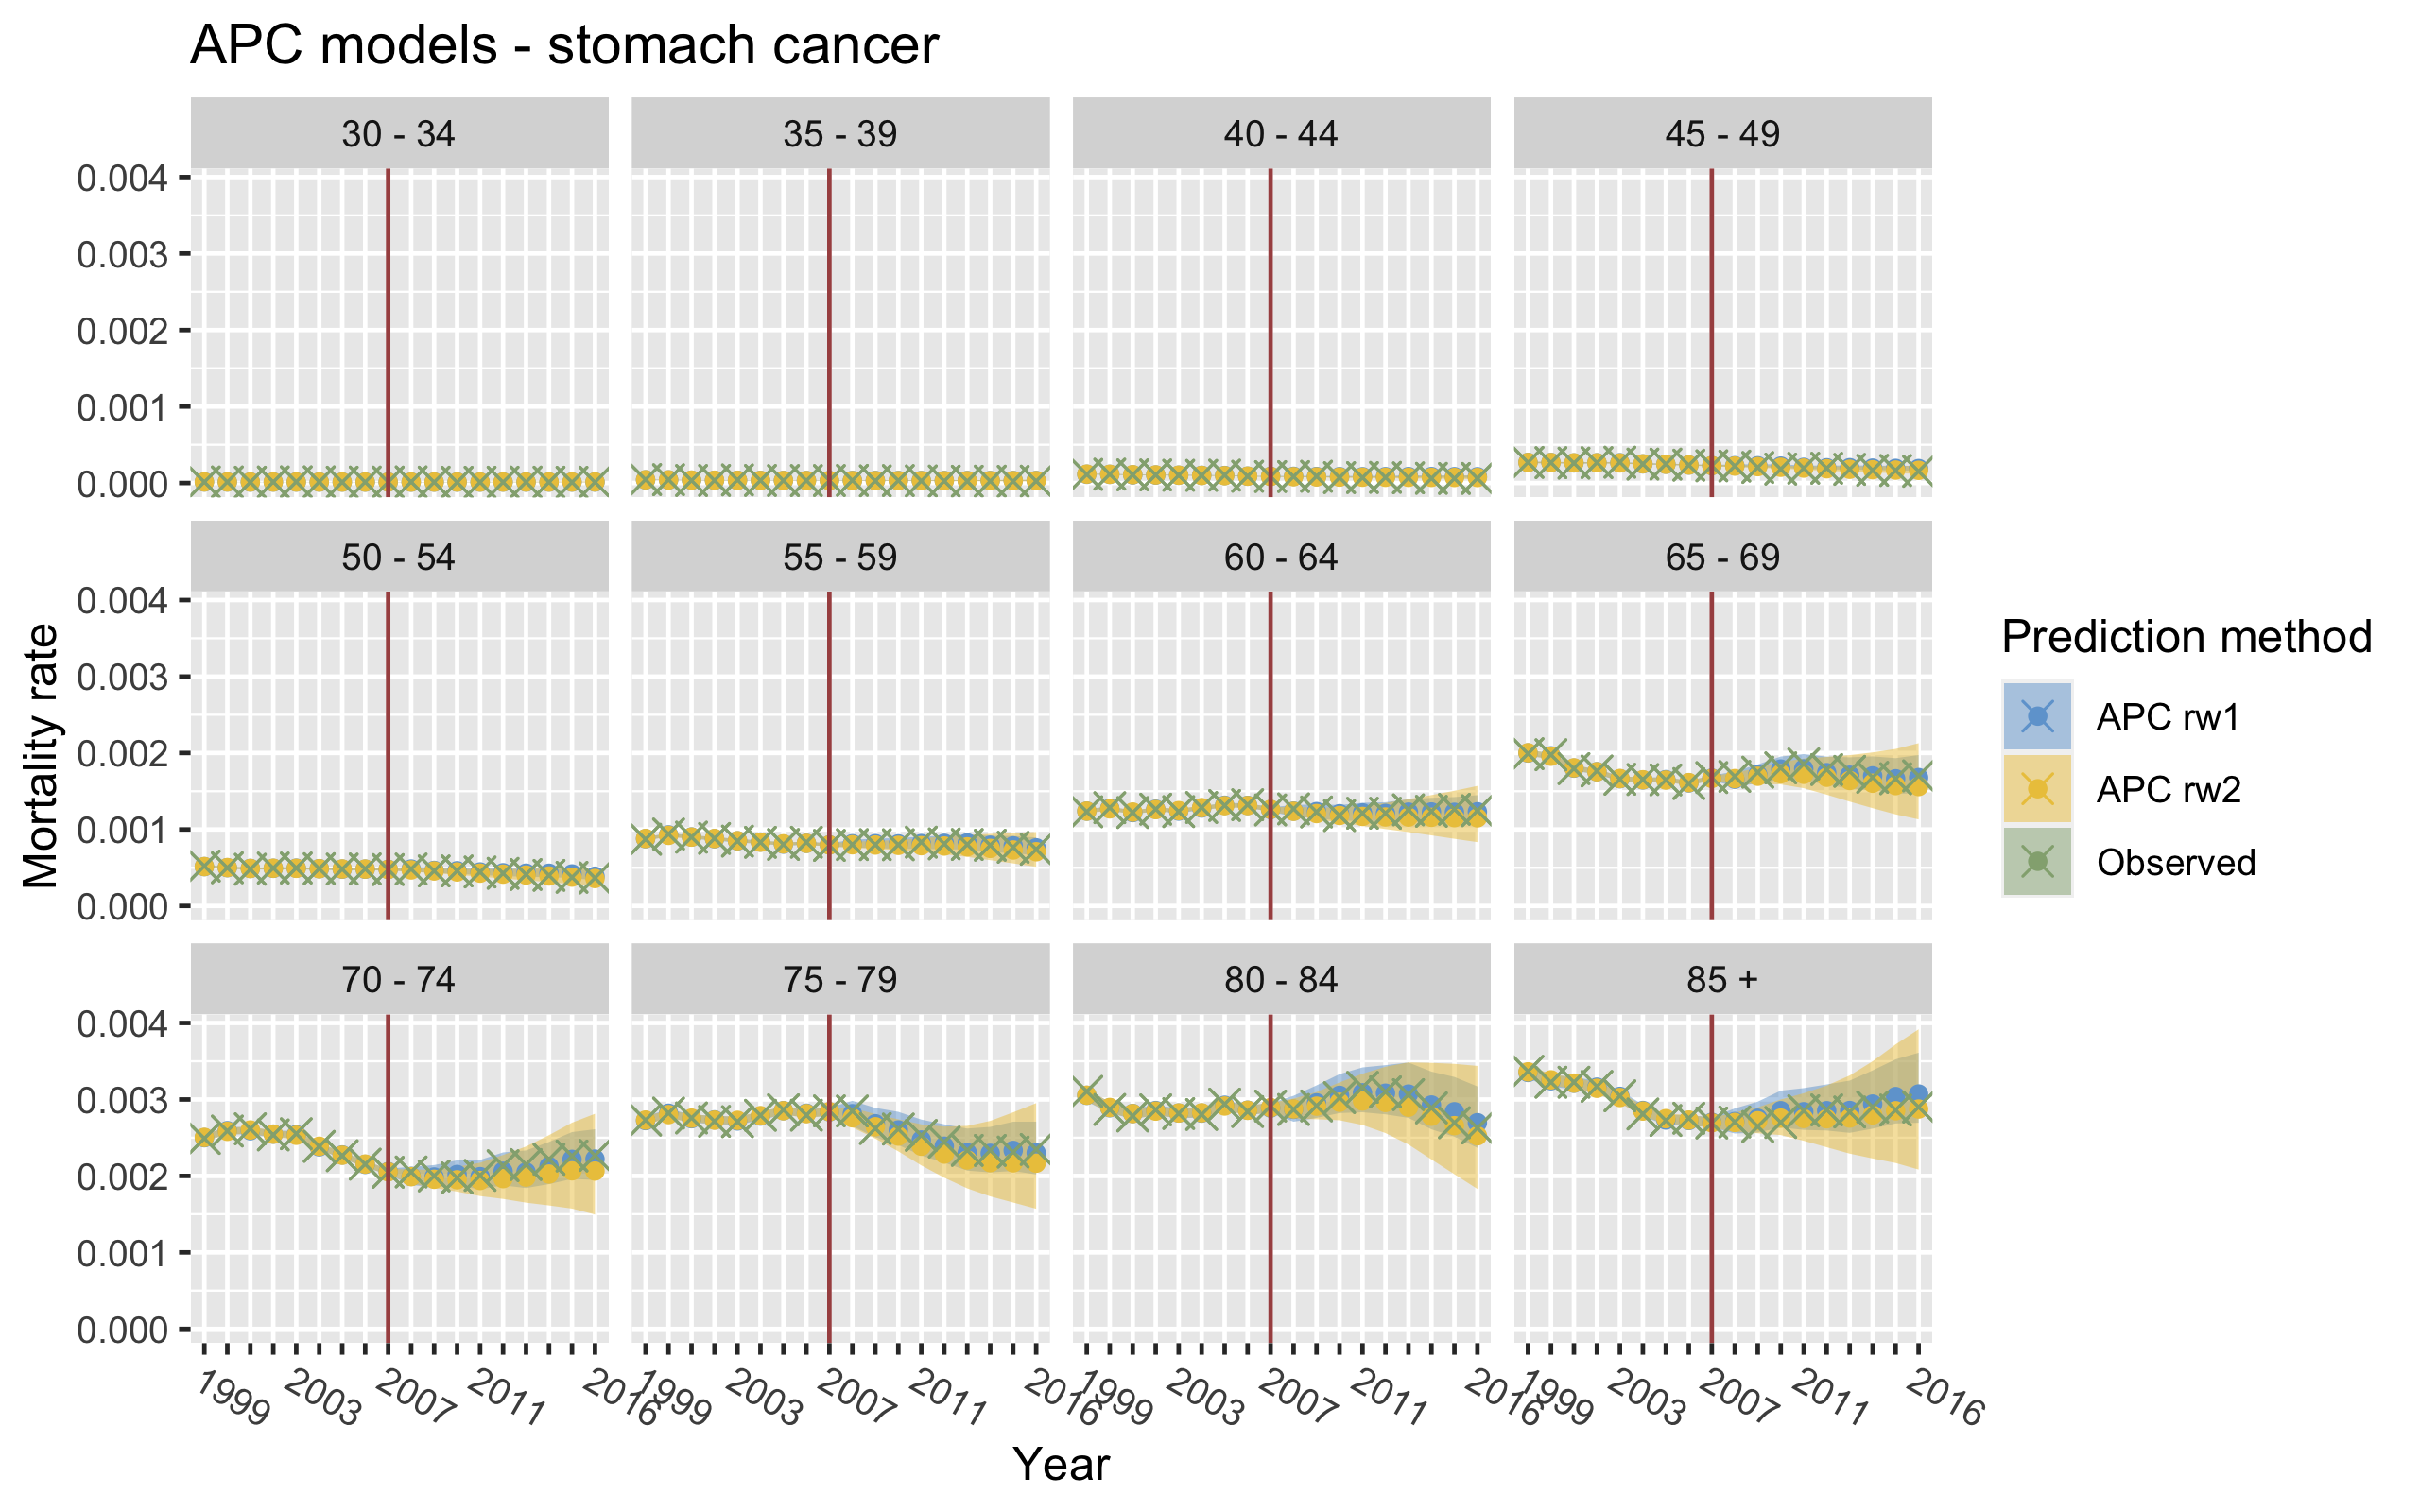
\includegraphics[width=\linewidth]{real-data/real-data-univariate/Figures/univariate-APC-by-period-stomach.png}
    \end{subfigure}
    \caption{Prediction results from inference with the APC types of models on the stomach cancer data set.}
    \label{fig:uv-APC-stomach}
\end{figure}

\begin{table}[h!]
    \begin{center}
        \begin{tabular}{l |c c c }
            Model & MSE &   MDSS & Contained 95\%-interval\\
            \hline
            APC1    & 2.591e-9 & -18.63    & 0.9383 \\
            APC2    & 7.774e-9 & -18.35    & 0.9877 \\
            LC         & 9.134e-8 & -12.60    & 0.4938 \\
            LCC        & 1.481e-8 & -17.99    & 0.9383 \\ 
            LCC-linear & 1.520e-8 & -17.89    & 0.8889 \\
        \end{tabular}
        \caption{Score statistics for different models applied to the stomach cancer data, calculated for predictions where $x > 8$.}\label{tbl:uv-stomach-8}
    \end{center}
\end{table}